\section{Spacecraft Modes of Operation}
The spacecraft will experience the following modes during its lifetime. A different configuration of system operations and instructions will be executed by \textit{SnapSat} in each case. These are summarised in below.

\noindent
\textbf{Launch Mode: } This turns the satellite off for launch to comply with CubeSat Design Specification 2.3.1. During launch the deployment switch is tripped which will turn the satellite on and transfer it into Establish Contact Mode. \\
\noindent
\textbf{Startup Mode: }This mode is entered only when the CubeSat is first launched.  In this mode the satellite will immediately turn on the ADCS to detumble.  Once the CubeSat is sufficiently stable (not tumbling in the pitch or roll axis) or 30 minutes has elapsed (CubeSat Design Specification 2.4.2) the antennas and solar panels will be deployed. It will then move into Standby Mode. \\
\noindent
\textbf{Standby Mode }In this mode, only essential satellite systems are kept ON.  This includes the OBC, EPS, VHF receiver,the GPS and intermittently the IMU.  It can transition out of Standby mode via an alert from the GPS, IMU, EPS or ground station orders.  \\
\noindent
\textbf{Payload Operation Mode: } This mode is used only when taking a picture and is entered through a location alert or ground station orders from Standby Mode.  The camera module is booted up, the camera takes a picture, stores it is RAM/ROM and then the camera is powered town again to conserve power.  After finishing these tasks it will return to Standby Mode. \\
\noindent
\textbf{Transmissions Mode: } This mode is entered once communications is established with the ground station or if the GPS acknowledges that a ground station is in range.  It will relay basic telemetry and if a picture is waiting in queue it will be sent.  If the EPS detects that the power is too low it will exit Transmissions mode, and will not allow it to enter it again until it has returned to acceptable levels.  Similarly the transmitter can be shut down by a command by the ground station.\\
\noindent
\textbf{Power Critical Mode: } In the event that the power level drops to a point where Standby is not sustainable SnapSat will enter this mode.  All systems will be turned off with the exception of the EPS for the purpose of charging the batteries.  It will exit this mode when the batteries are sufficiently charged. \\
\noindent
\textbf{De-tumble mode: } This mode is used to de-tumble the spacecraft after deplopment into orbit as well as to recover it from any spin states (such as after Safe Mode). All Safe Mode components are ON, as well as the ADCS system. Other devices can be turned ON by ground command without a change of state. \\

\noindent
\tikzstyle{block} = [rectangle, draw, line width=1pt, fill=none, 
text width=3cm, text centered, rounded corners, minimum height=1cm]
\tikzstyle{green} = [rectangle, draw, fill=none, 
text width=3cm, text centered, line width=1pt, fill=green!10, rounded corners, minimum height=1cm]
\tikzstyle{line} = [draw, -latex', line width=1pt]

\begin{figure}[H] \centering
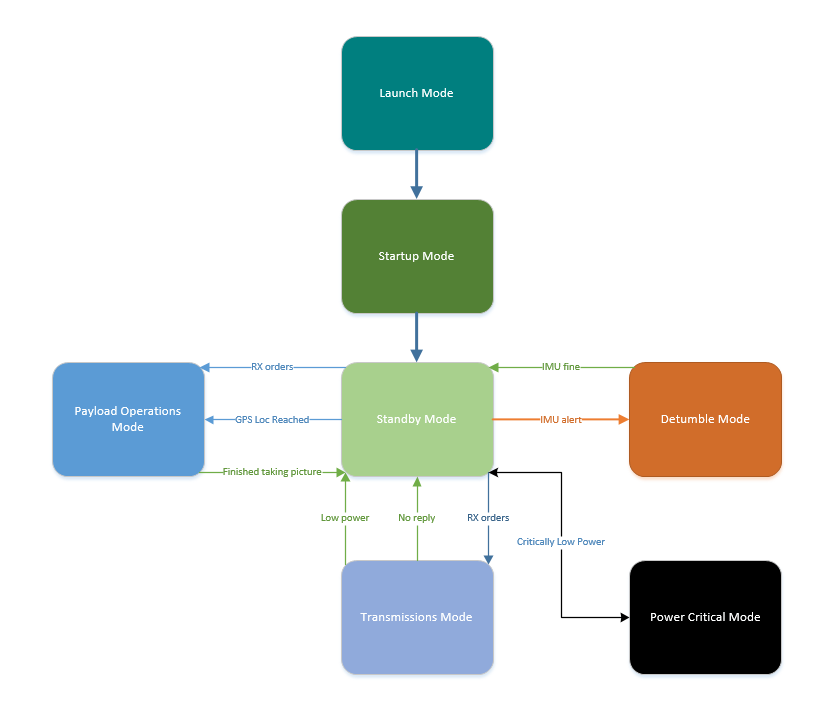
\includegraphics[width=\textwidth]{States.png}
\caption{Mode Transition Diagram during satellite lifetime}
\end{figure}

